%!TEX root = ./main.tex
\section{Implementation}
\label{sec4}

Our lightweight approach of resugaring is implemented using PLT Redex\cite{SEwPR}, which is an semantic engineering tool based one reduction semantics. The whole framework is as Fig\ref{fig:frame}.

\begin{figure}[h]
	\centering
	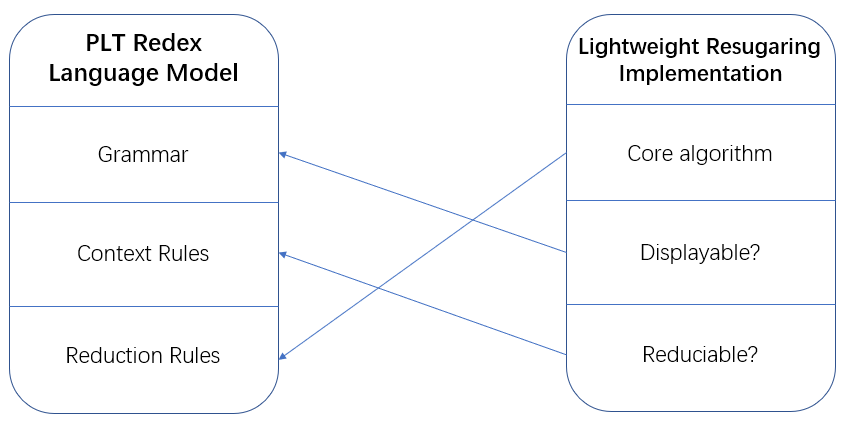
\includegraphics[width=12cm]{images/frame.png}
	\caption{framework of implementation}
	\label{fig:frame}
\end{figure}

The grammar of the whole language contains Coreexp, Surfexp and Commonexp as the language setting in sec\ref{sec3}. OtherSurfexp is of Surfexp and OtherCommonexp is of Commonexp. The identifier of any kind of expression is Headid of expression. If we need to add a syntactic sugar to the whole language, only three steps is needed.

\begin{enumerate}
\item Add grammar of the syntactic sugar.
\item Add context rules of the sugar, such that any sub-expressions can be reduced.
\item Add desugar rules of the sugar to reduction rules of the whole language.
\end{enumerate}

Then inputting an expression of the syntactic sugar to lightweight-resugaring will get the resugaring sequences.